% !TEX root = EUDAQUserManual.tex
\section{Introduction}
The EUDAQ software is a data acquisition framework, written in C++,
and designed to be modular and portable, running on Linux, Mac OS X, and Windows.
It was written primarily to run the EUDET Pixel Telescope\cite{Roloff:2009zza},
but is designed to also be generally useful for other systems.

The hardware-specific parts are kept separate from the rest,
so that the common parts can still be used independently.
These include software for accessing the \gls{TLU} and the \gls{EUDRB} used by the EUDET beam telescope.

The data files generated by the DAQ can be easily converted to the \gls{LCIO} format,
allowing the data to be analysed with the EUTelescope\cite{eutel2008} analysis package.

\subsection{Architecture}
It is split into a number of different processes (see \autoref{fig:DAQ}),
each communicating using TCP sockets.
A central Run Control provides an interface for controlling the whole DAQ system;
other processes connect to the Run Control to receive commands and to report their status.

\begin{figure}[htb]
  \begin{center}
    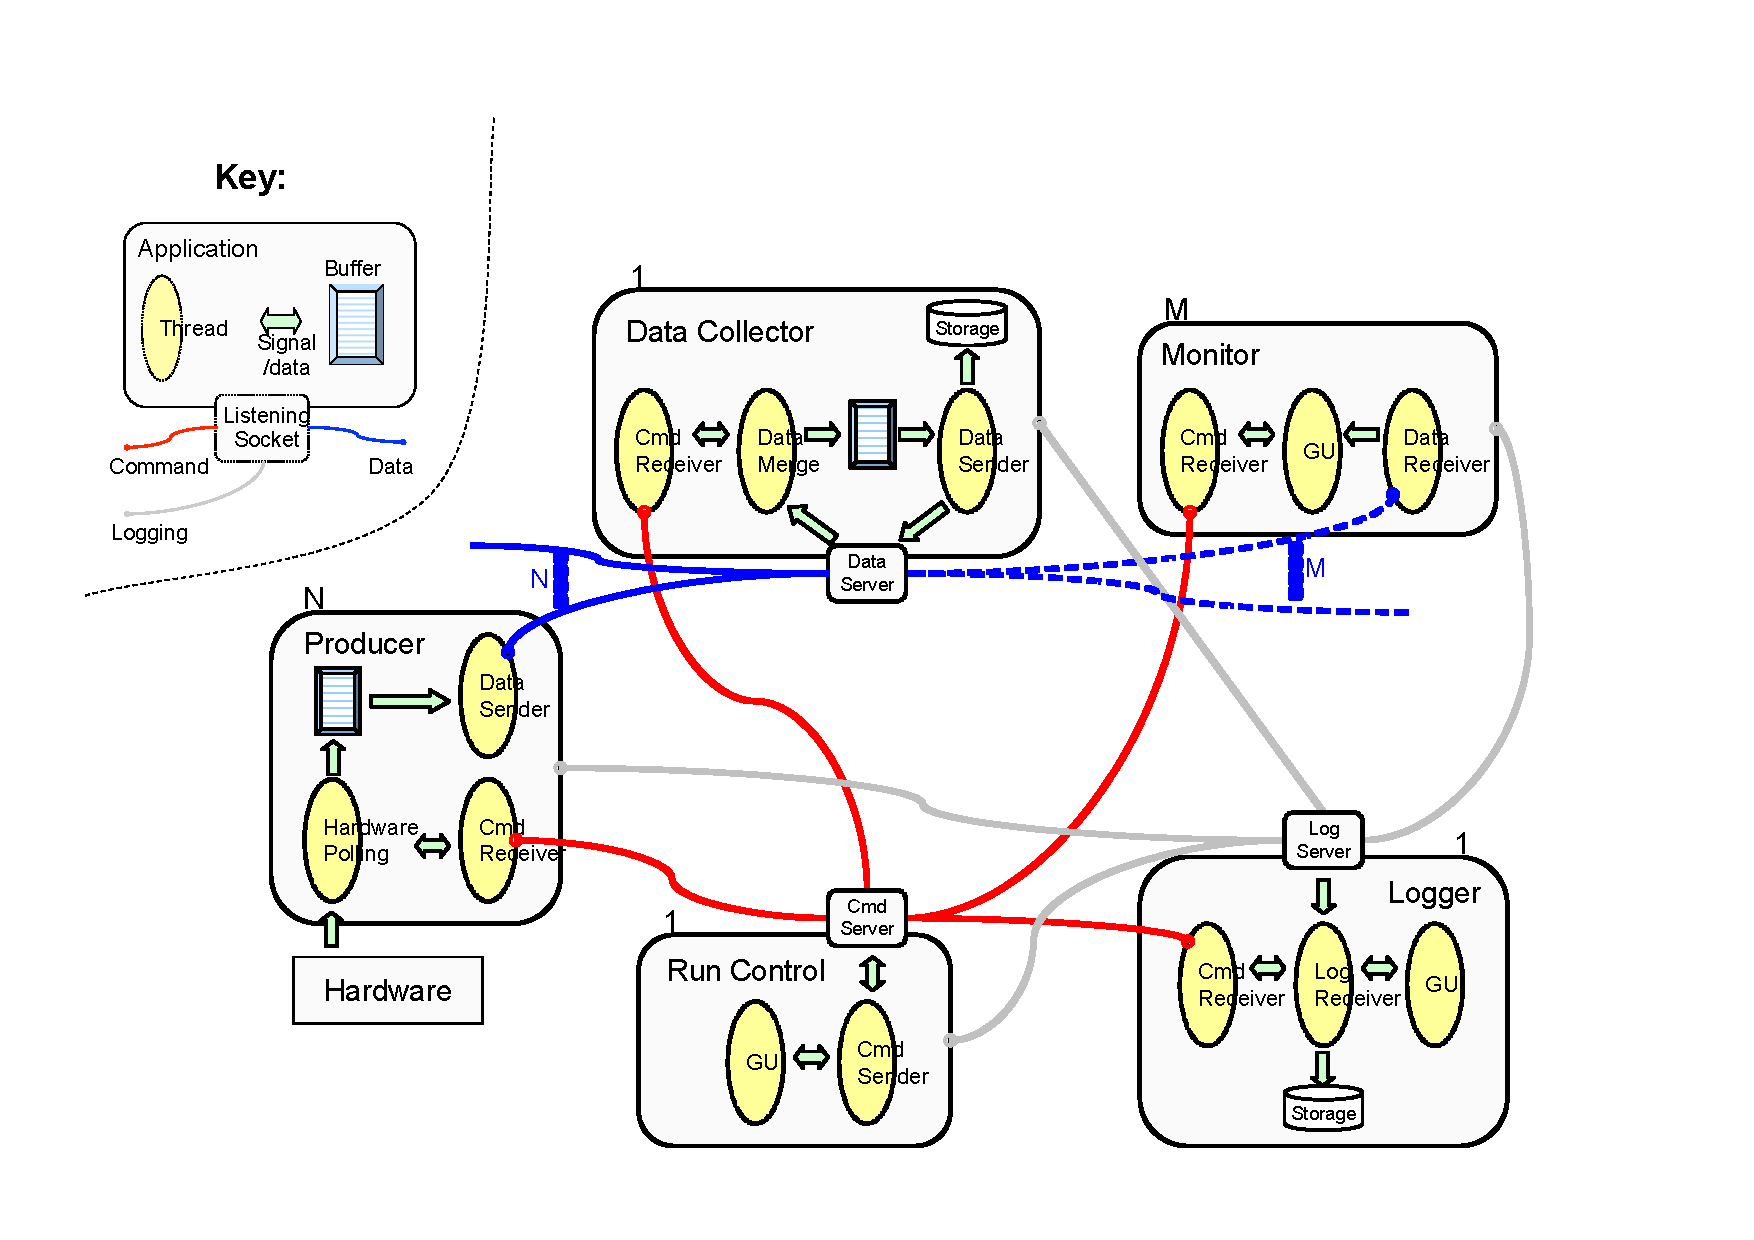
\includegraphics[width=0.9\textwidth]{DAQ}
    \caption{Schematic of the DAQ architecture.}
    \label{fig:DAQ}
  \end{center}
\end{figure}

Each piece of hardware that produces data (e.g. the \gls{TLU}, the telescope, or a \gls{DUT}) will have a Producer process.
This will configure the hardware, read out the data and send it to the Data Collector.

The Data Collector receives all the data streams from all the Producers,
and combines them into a single stream that is written to disk.
It usually writes the data in a native raw binary format,
but it can be configured to write in other formats, such as \gls{LCIO}.

The Logger receives log messages from all other processes,
and displays them to the user, as well as writing them all to file.
This allows for easier debugging, since all log messages are stored together in a central location.

A Monitor reads the data file and generates online-monitoring plots for display.
In the schematic it is shown to communicate with the DataCollector via a socket,
but it actually just reads the data file from disk (this may be changed in the future).

\subsection{Directory Structure}
The EUDAQ software is split into several parts that can each be compiled independently,
and are kept in separate subdirectories.
The general structure is outlined below:

\begin{myitemize}
\item \texttt{main}
  contains the main EUDAQ library with the parts that are common to most of the software,
  and several command-line programs that depend only on this library.
  All definitions in the library should be inside the \texttt{eudaq} namespace.
  It is organised into the following subdirectories:
  \begin{myitemize}
  \item \texttt{lib/src}
    contains the library source code,
  \item \texttt{exe/src}
    contains the (command line) executables source code,
  \item \texttt{include}
    contains the header files inside the \texttt{eudaq} subdirectory (to match the namespace),
  \end{myitemize}
\item \texttt{gui}
  contains the graphical programs that are built with Qt, such as the RunControl and LogCollector.
\item \texttt{producers}
  contains all (user-provided) producers shipped with the EUDAQ
  distribution, for example:
  \begin{myitemize}
\item \texttt{tlu} and \texttt{eudrb}
  contain the parts that depend on the \gls{TLU} and \gls{EUDRB} respectively.
\item\texttt{vme}
  contains a wrapper for the VME driver for the \gls{EUDRB}.
\item \texttt{depfet}, \texttt{fortis}, \texttt{taki}\ldots{}
  contain the code for third-party producers that have been used with
  the telescope.
  \end{myitemize}
\item \texttt{extern}
  stores external software that is not part of EUDAQ itself, but that is needed by EUDAQ in some cases,
  such as the ZestSC1 driver for the \gls{TLU} and the Tsi148 VME driver.
\item \texttt{bin} and \texttt{lib}
  contain the compiled binaries (executables and libraries) generated from the other directories.
\item \texttt{conf}
  contains configuration files for running the beam telescope.
\item \texttt{data} and \texttt{logs}
  are directories for storing the data and log files generated while running the DAQ.
\item \texttt{doc}
  contains documentation, such as this manual.
\end{myitemize}

Each directory containing code has its own \texttt{src} and \texttt{include} subdirectories,
as well as a local \texttt{CMakeLists.txt} file containing the rules
for building that directory using \texttt{CMake}.
Header files usually have a \texttt{.hh} extension so that they can be automatically recognised as C++
(as opposed to C), and source files have either \texttt{.cc} for parts of a library or \texttt{.cxx} for executables.
